\chapter{Image Acquisition and Calibration}

Images need to be acquired before they can be calibrated.\\

Since cross-talk between channels cannot be eliminated completely, there needs to be two cameras due to the Bayer matrix colour array. Attempts to use a single camera is not as effective as a dual-camera setup as explained in Section \ref{sec:filters}.\\

The idea is also to use cost-effective technology, and thus the 8 MP Sony IMX219 series cameras will be used since they integrate easily with the Raspberry Pi using single 15-pin CSI connections.\\

%The following concepts are crucial to understand the reasoning behind certain decisions.\\

In consumer cameras, the filter pattern is arranged in an RGGB format as in Figure \ref{fig:bayer}, to mimic the physiology of the eye. Demosiacing is performed to interpolate the neighbouring pixel colours for every pixel.

\begin{figure}[H]
\centering
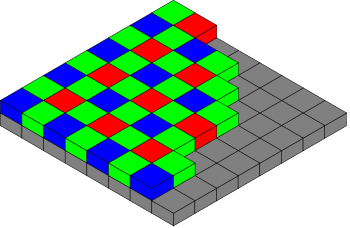
\includegraphics[scale=0.35]{images/bayer.png}
\caption{Bayer arrangement of colour filters on an image sensor's pixel array \cite{bayer}}
\label{fig:bayer}
\end{figure}

The colour filters do allow infra-red light in as well, which is why consumer cameras generally have a NIR longpass filter in place to isolate RGB colours. Even then it cannot block strong sources of NIR light from hitting the sensor as in Figure \ref{fig:ir_escape}.

\begin{figure}[H]
\begin{subfigure}{0.5\textwidth}
\centering
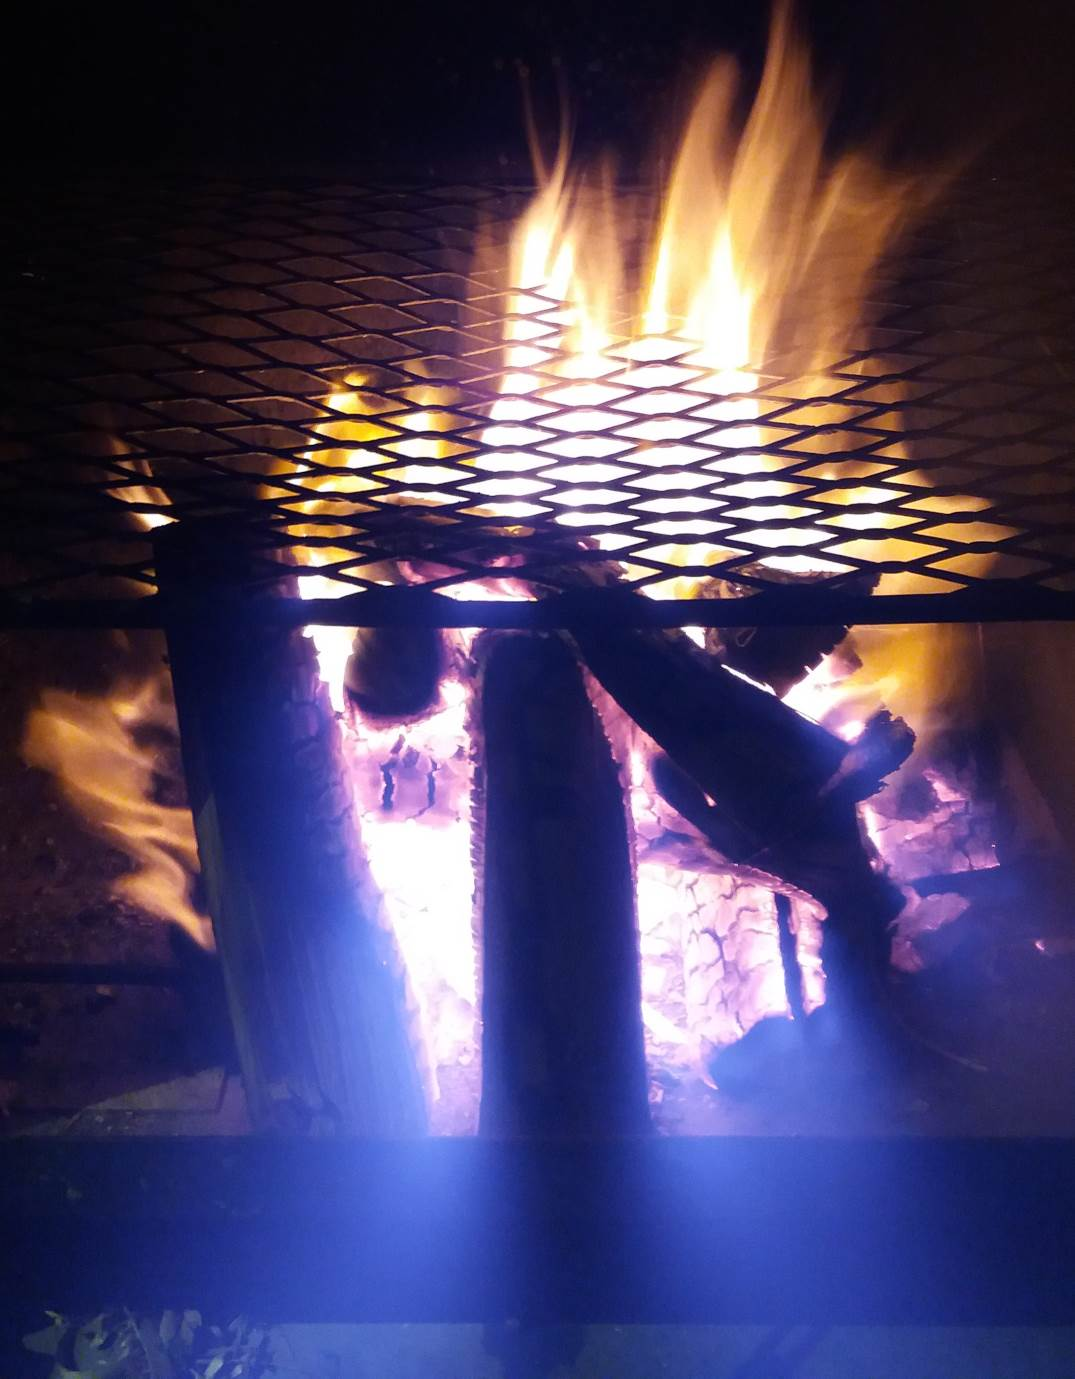
\includegraphics[scale=0.2]{images/fire_ir.jpg}
\caption{NIR light escaping from a fire}
\label{fig:fire_ir}
\end{subfigure}
\begin{subfigure}{0.5\textwidth}
\centering
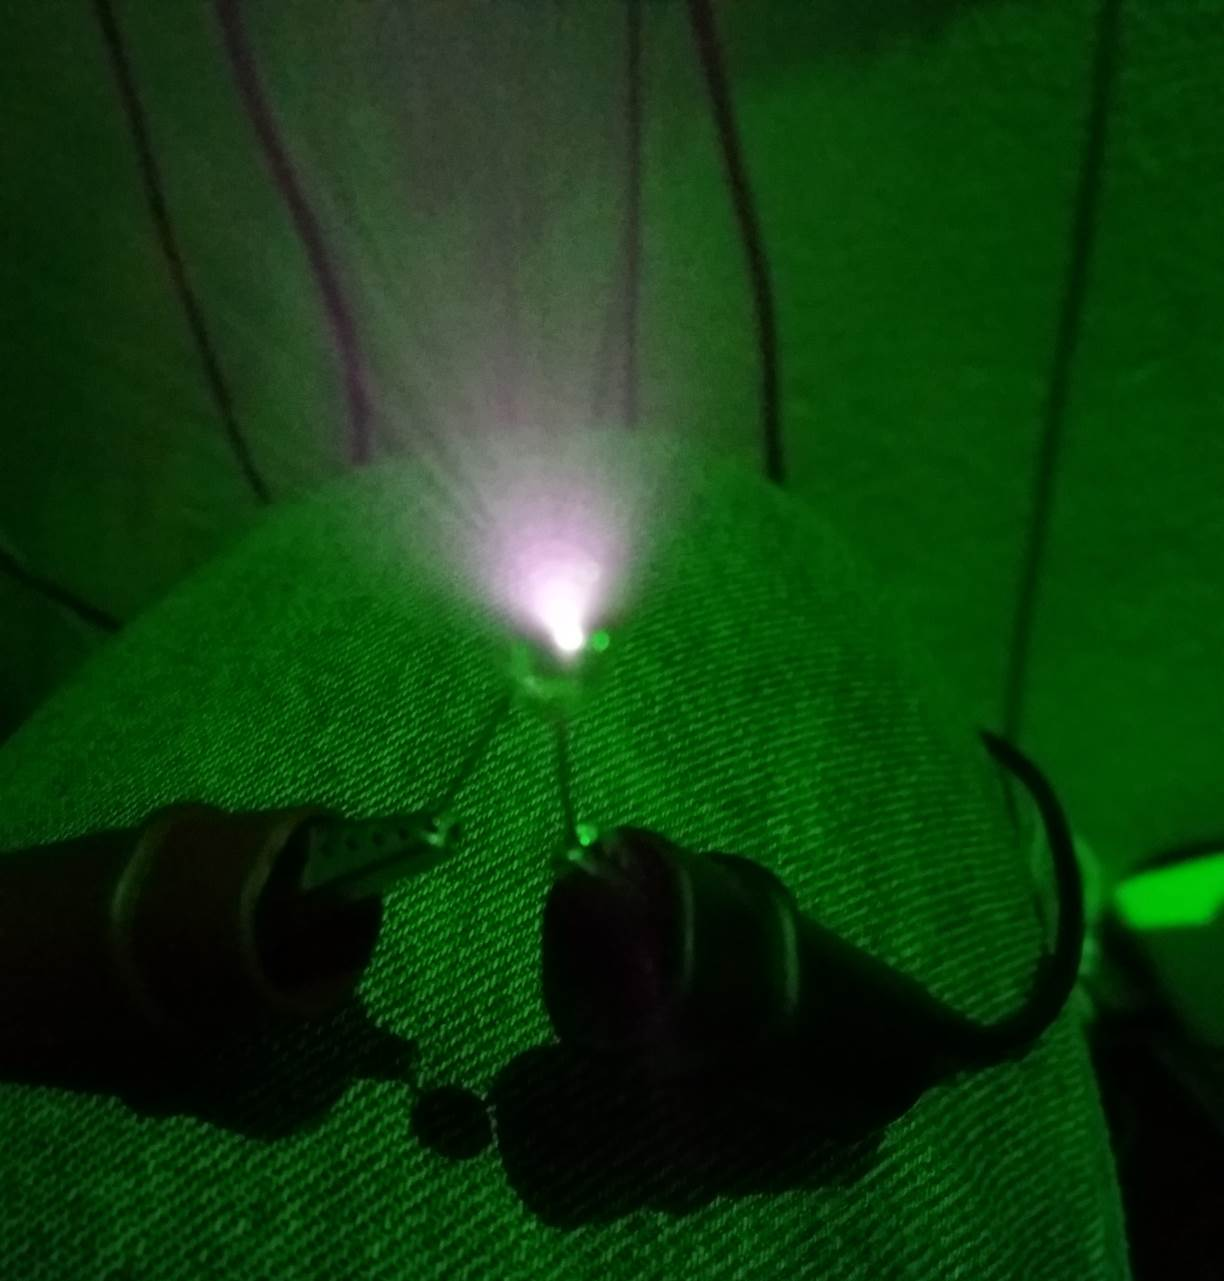
\includegraphics[scale=0.219]{images/ir_led.jpg}
\caption{A single NIR LED.}
\end{subfigure}
\caption{In this case, a cellphone camera picking up NIR light.}
\label{fig:ir_escape}
\end{figure}

Due to variances in focal length, and slight manufacturing disparities, there is some rotation and translation in real lenses.\\

There is also distortion, as in Figure \ref{fig:distortion_examples}, which will be dealt with from Section \ref{sec:cam_model} onwards.

\begin{figure}[H]
\centering
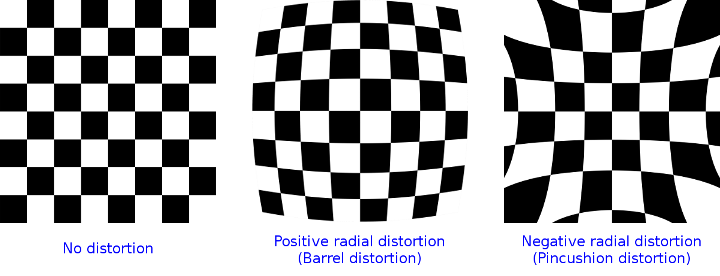
\includegraphics[scale=0.5]{images/distortion_examples.png}
\caption{Distortion examples \cite{calib3d}}
\label{fig:distortion_examples}
\end{figure}

This can be modelled by the pinhole camera model as in Section \ref{sec:pinhole}.

%\subsection{Camera Calibration}
%
%(picture of undistortion).
%
%\subsubsection{Jello effect}
%
%ripple


\section{Filters}
\label{sec:filters}

One of the big questions asked is whether two cameras are needed? Can one not just use a filter on a single camera? The differences between a single and dual camera setup is shown in Appendix \ref{app:filter_comparison}. The comparison uses blue, green, red and no filter. Perhaps the biggest difference that one can notice is that the fence, swing and other objects are `green' and healthy in the single setup, which shows that, indeed, the NIR light is not completely separated from the visible light. Also, due to the colour LUT, green, yellow, orange, and red show a respectively greater ratio of infrared light to visible light. And yes, this red colour (or strong infrared to visible light ratio) is more visible in the dual camera setup. The dual camera setup also shows a greater variance, and it can be deduced that it has a greater chance of actually determining healthy plants from otherwise. Lastly, all three filters show good separation from infrared light, and thus the blue filter was used due to simplicity (the material is a type of film, not glass).\\

%A filter is needed to isolate the NIR channel. If a custom filter is used on a camera with the NIR filter removed, it is possible to isolate a NIR channel without visible light leakage. A few of the variants include the Wratten 25A Red Long Pass filter, the Wratten 87 NIR All Pass filter and the Rosco 2008 Blue filter, which allow red and NIR light, only NIR light, and blue and NIR light respectively.\\

The blue filter is a Rosco 2008, the red filter is a 600nm Dichroic Glass Longpass filter and the green filter is a 500nm Dichroic Glass Bandpass filter from Edmund Scientific.\\

The blue filter in Figure \ref{fig:blue_filter} passes only NIR light within the green and red channels, as shown in Figure \ref{fig:blue_curve}.

\begin{figure}[H]
\begin{subfigure}{0.5\textwidth}
\centering
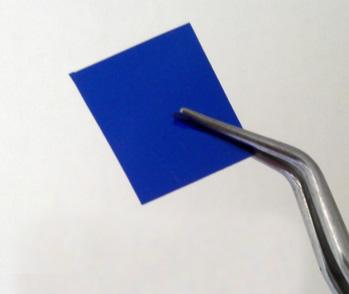
\includegraphics[scale=0.45]{images/blue_filter.jpg}
\caption{Blue Rosco 2008 filter \cite{blue_filter}}
\label{fig:blue_filter}
\end{subfigure}
\begin{subfigure}{0.5\textwidth}
\centering
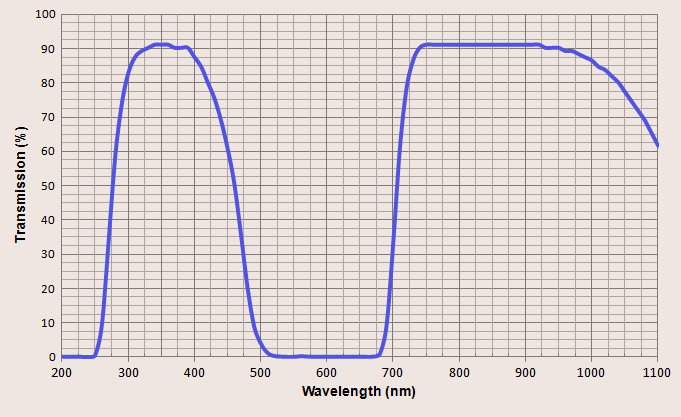
\includegraphics[scale=0.42]{images/superblueinfraredfiltercurve.png}
\caption{Blue filter transmission curve.}
\label{fig:blue_curve}
\end{subfigure}
\caption{Blue filter characteristics \cite{blue_curve}}
\label{fig:blue_character}
\end{figure}

%\begin{figure}[H]
%\centering
%	
%\subfloat[Blue Rosco 2008 filter \cite{blue_filter}]
%	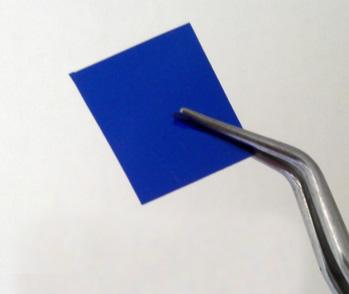
\includegraphics[scale=0.45, width=0.5\textwidth]{images/blue_filter.jpg}
%	\label{fig:blue_filter2}
%
%	
%\subfloat[Blue filter transmission curve.]
%	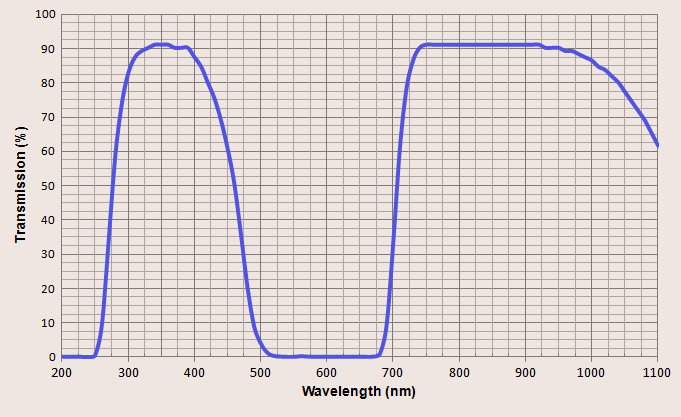
\includegraphics[scale=0.42]{images/superblueinfraredfiltercurve.png}
%	\label{fig:blue_curve2}
%
%\caption{Blue filter characteristics \cite{blue_curve}}
%\label{fig:blue_characte2r}
%\end{figure}
%
%\section{Cameras}

%It is seemingly impossible to capture pure NIR and pure red on separate channels unless the intrinsic bayer matrix is manufactured to allow for it, however, then it would not be cost effective (citation needed).\\

\section{Exposure}

It is important that the correct white-balance settings are chosen so as not to allow extremeties such as in Figure \ref{fig:exposure} to occur.

\begin{figure}[H]
\begin{subfigure}{0.5\textwidth}
\centering
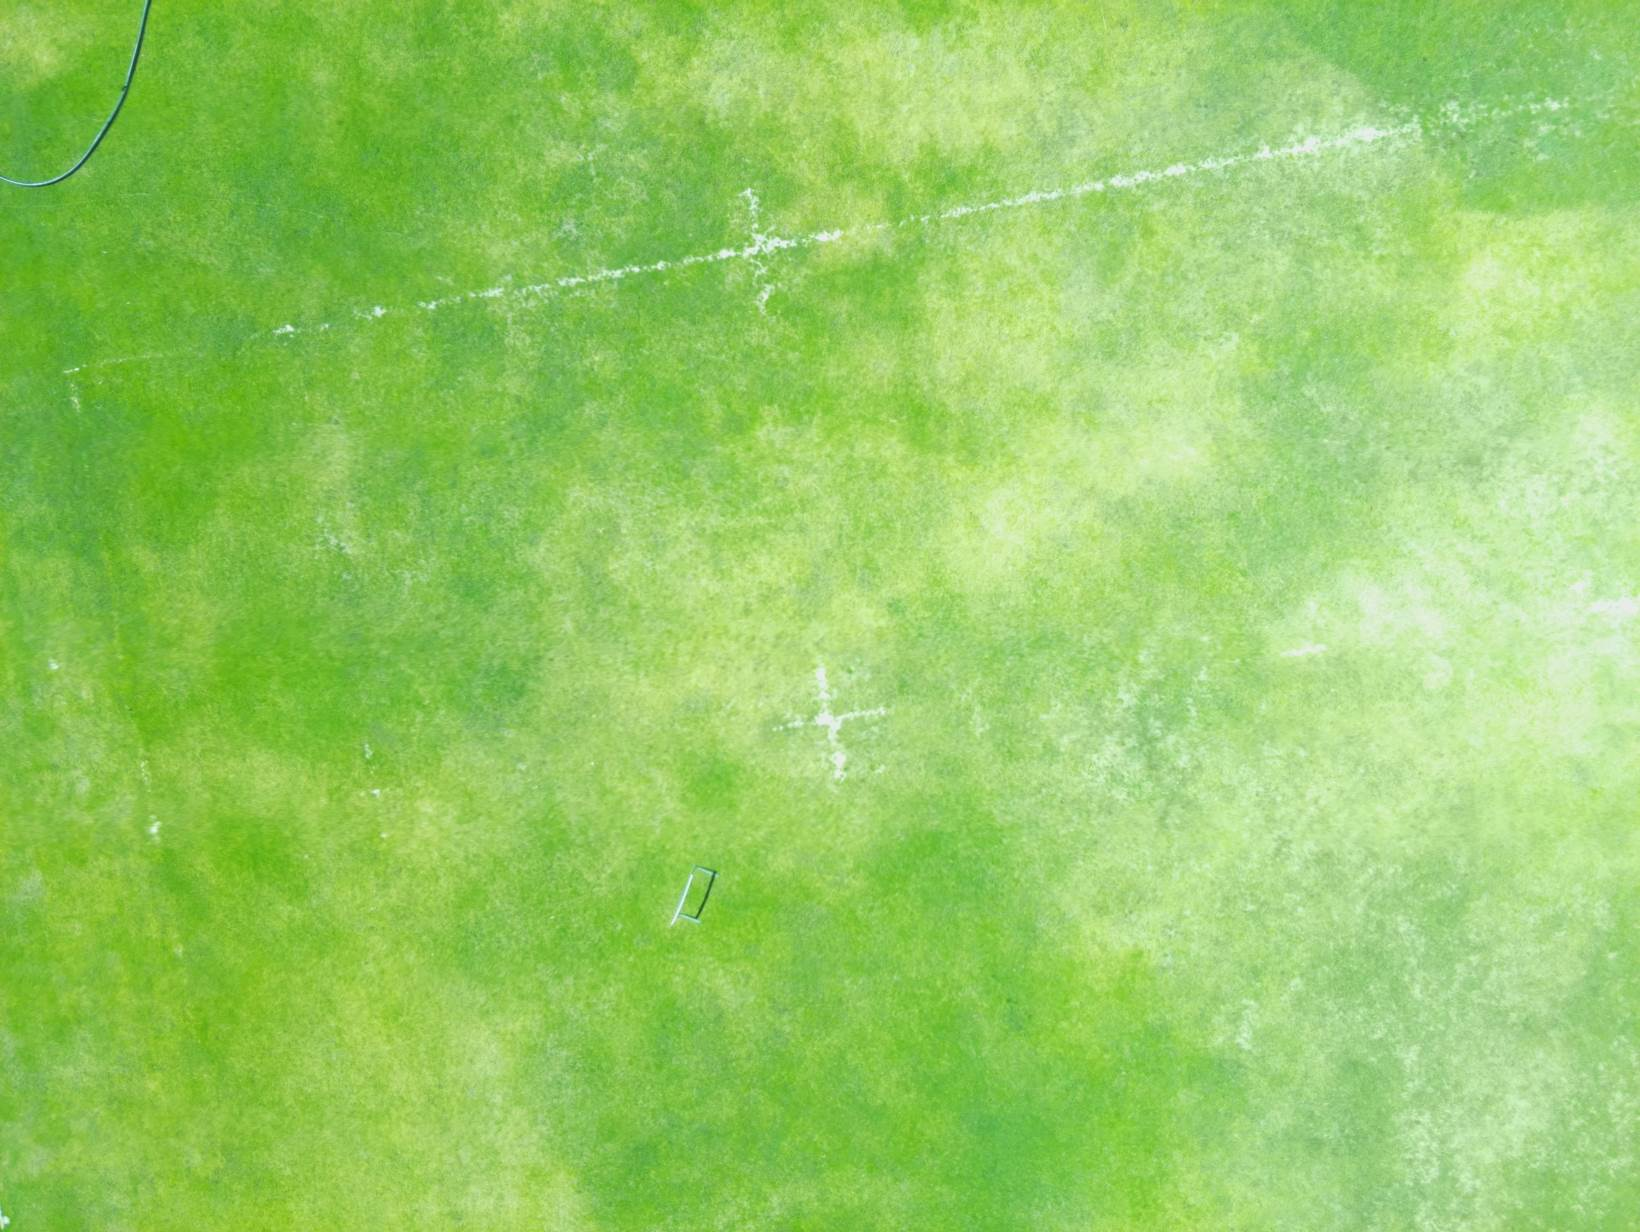
\includegraphics[scale=0.17]{images/under-exposed.jpg}
\caption{Under exposed}
\label{fig:under_exposed}
\end{subfigure}
\begin{subfigure}{0.5\textwidth}
\centering
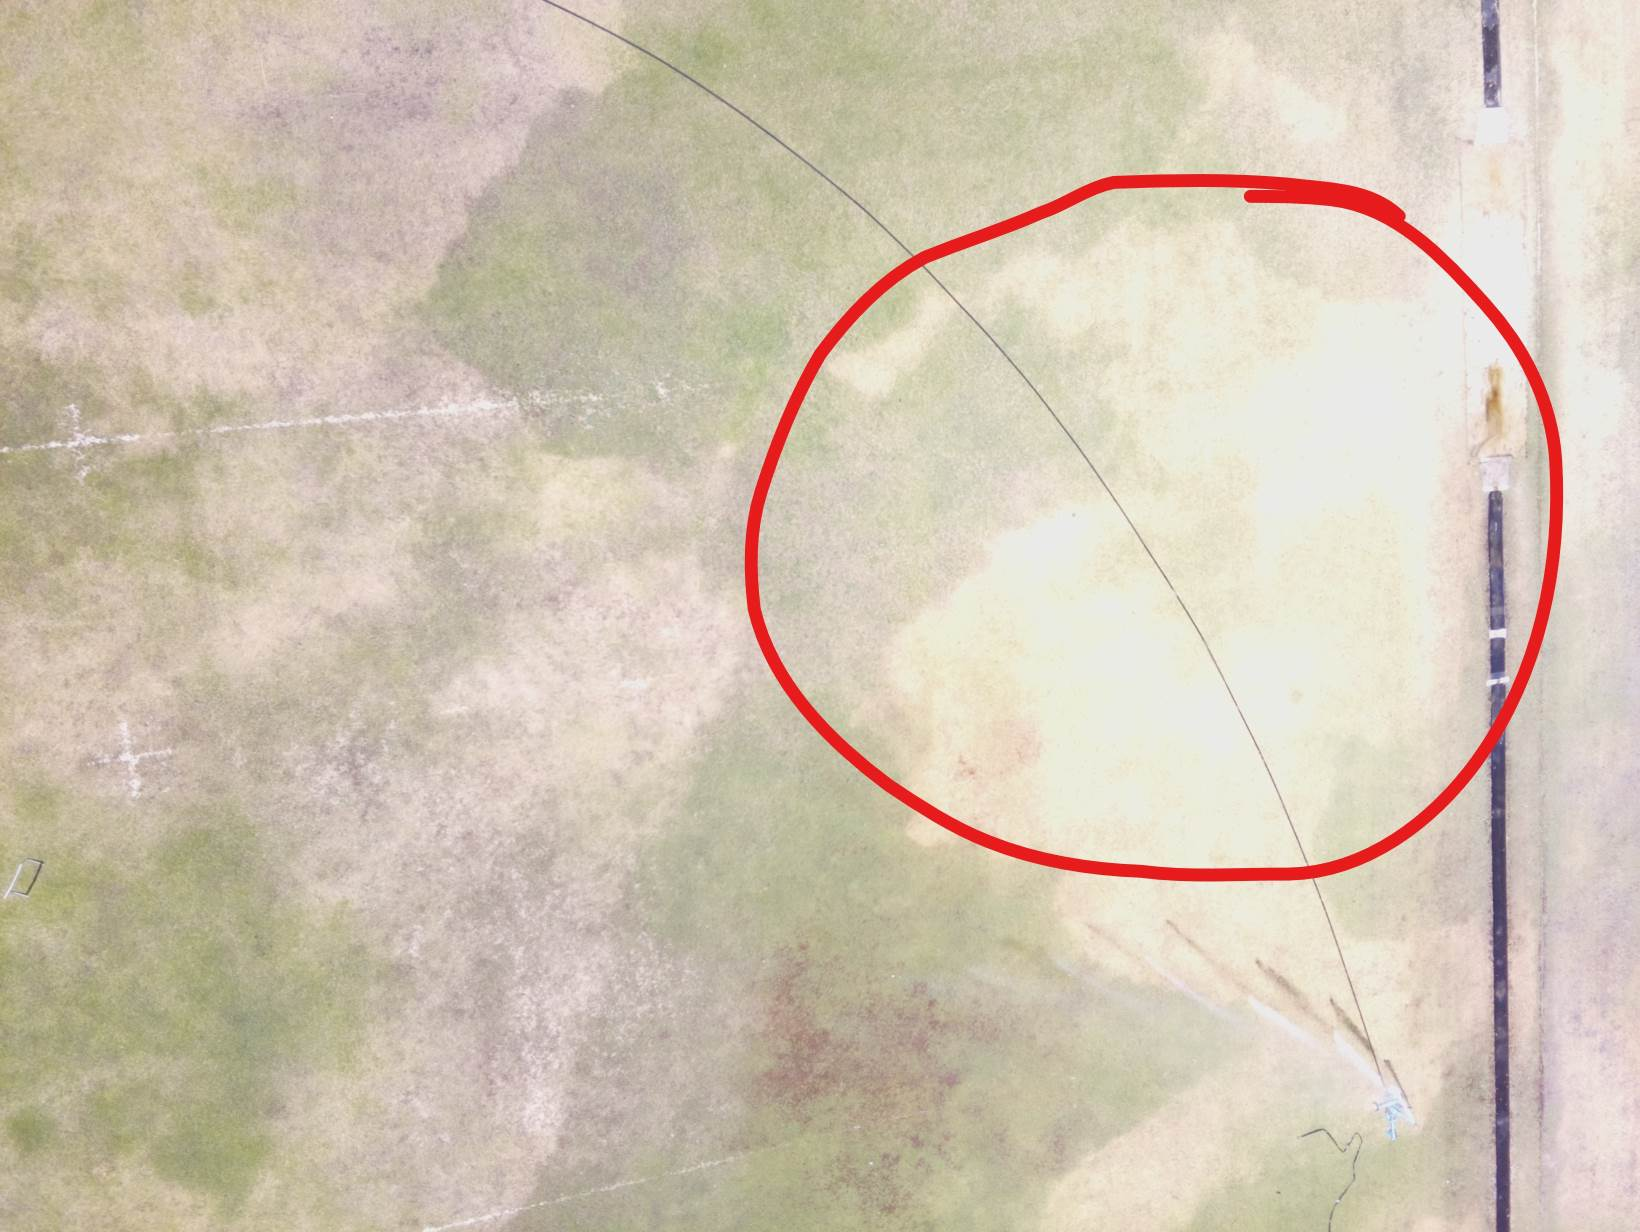
\includegraphics[scale=0.17]{images/over-exposed.jpg}
\caption{Over exposed}
\label{fig:over_exposed}
\end{subfigure}
\caption{Incorrect exposure settings}
\label{fig:exposure}
\end{figure}

A calibration plate as in Section \ref{sec:cal_plate} should resolve drift in NDVI values caused by clouds or sunshine, although glare might be more of an issue.

\section{Camera mount}

The motors cause high-frequency vibrations, and if not removed, it can cause what is known as the Jello-effect as in Figure \ref{fig:jello_effect}. It is also as a result of the cameras use a rolling shutter and not a global/mechanical shutter, which is more expensive.

\begin{figure}[H]
\centering
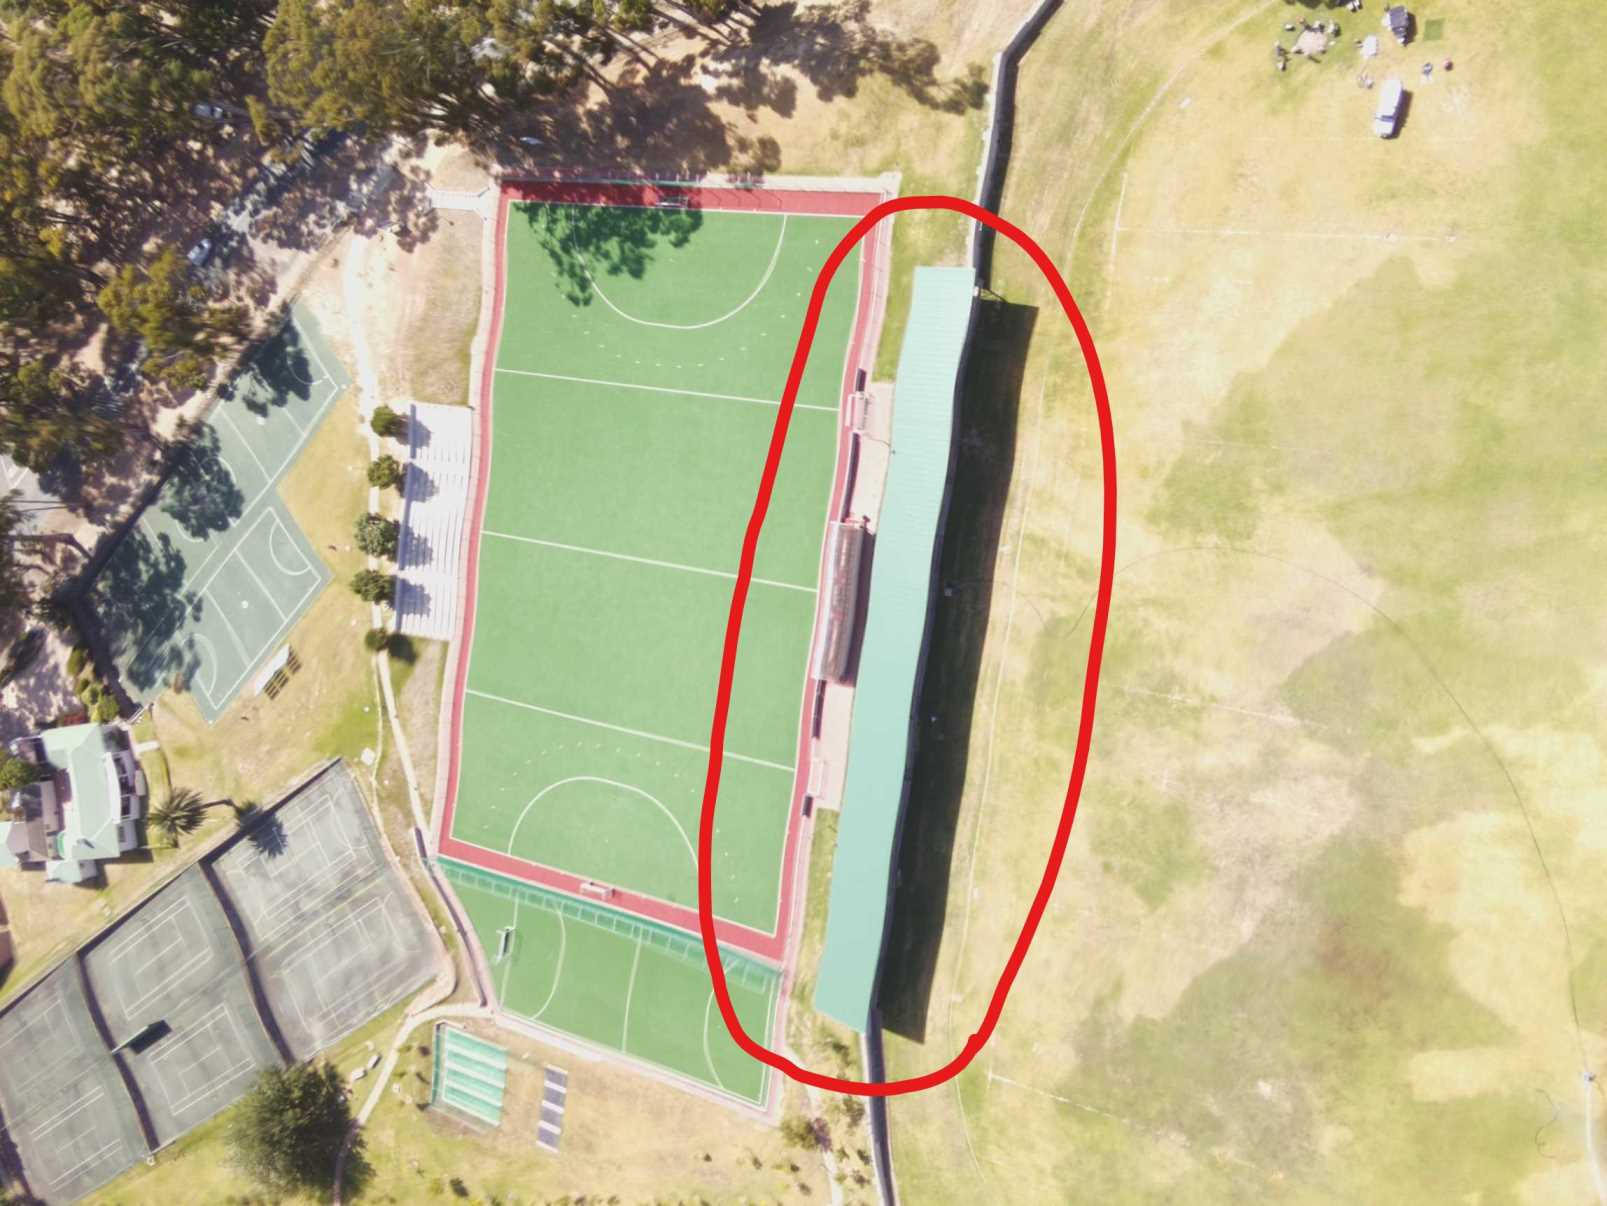
\includegraphics[scale=0.27]{images/ripple.jpg}
\caption{Jello-effect visible before dampening}
\label{fig:jello_effect}
\end{figure}

To fix the Jello-effect, an attempt was made as in Figure \ref{fig:moon_gel} by using Moongel. Moongel is used by drummers, on cymbols and drumheads to diminish overtones, and has damping properties. It showed good damping in lateral directions, but much less vertically, thus overall it did not make much difference.

\begin{figure}[H]
\centering
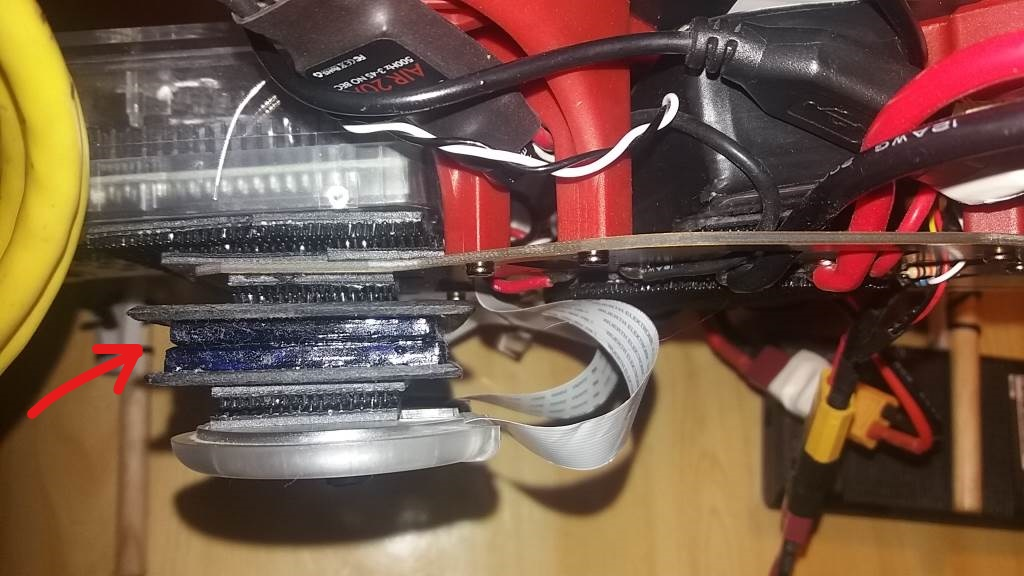
\includegraphics[scale=0.27]{images/moon_gel.jpg}
\caption{Moongel platform}
\label{fig:moon_gel}
\end{figure}

Another attempt was made using cable-ties as in Figure \ref{fig:dampener} which allowed damping in any direction. This proved to be effective.\\

The cameras are fixed relative to each other using a PCB substrate so that no rotational or translational drift can occur as in Figure \ref{fig:cam_mount}.\\

\begin{figure}[H]
\begin{subfigure}{0.5\textwidth}
\centering
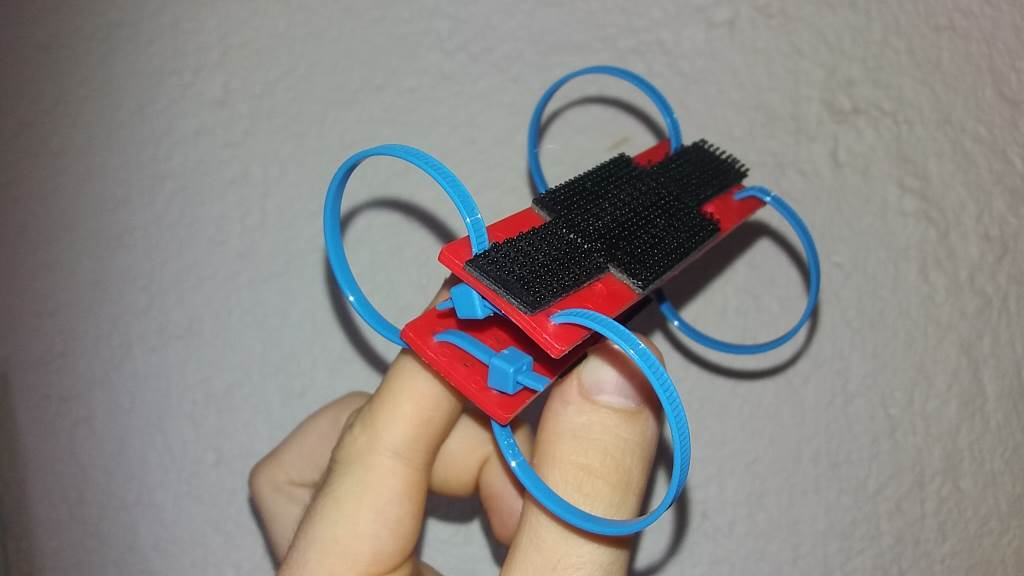
\includegraphics[scale=0.3]{images/dampener.jpg}
\caption{Dampening for the cameras}
\label{fig:dampener}
\end{subfigure}
\begin{subfigure}{0.5\textwidth}
\centering
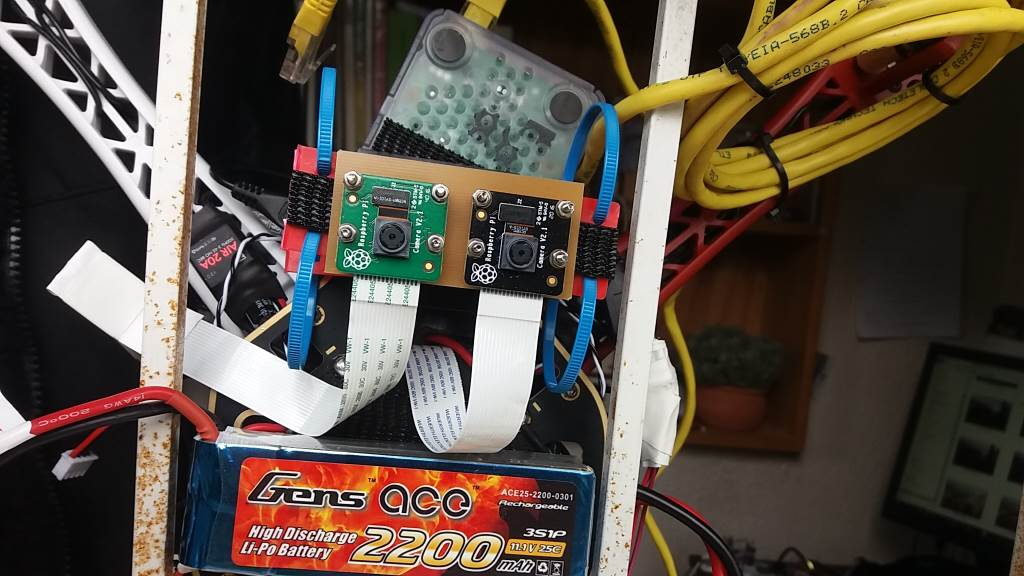
\includegraphics[scale=0.3]{images/fixed_orientation.jpg}
\caption{Fixed orientation for cameras}
\label{fig:fixed_orientation}
\end{subfigure}
\caption{Camera mount}
\label{fig:cam_mount}
\end{figure}

Although a DC brushless motorised gimbal would aid in nadir orientation, increasing the overlap between images should account for when the cameras are not pointing directly downwards.

\section{Simultaneous triggering}
\label{sec:simultaneous_trig}

Initially, an IVmech Camera multiplexer was used as in Figure \ref{fig:ivmech}. Unfortunately, it didn't work. Upon debugging using a logic analyser, the $CAM\_GPIO$ and $CAM1\_DN$ pins were not multiplexed as they should have been.

\begin{figure}[H]
\centering
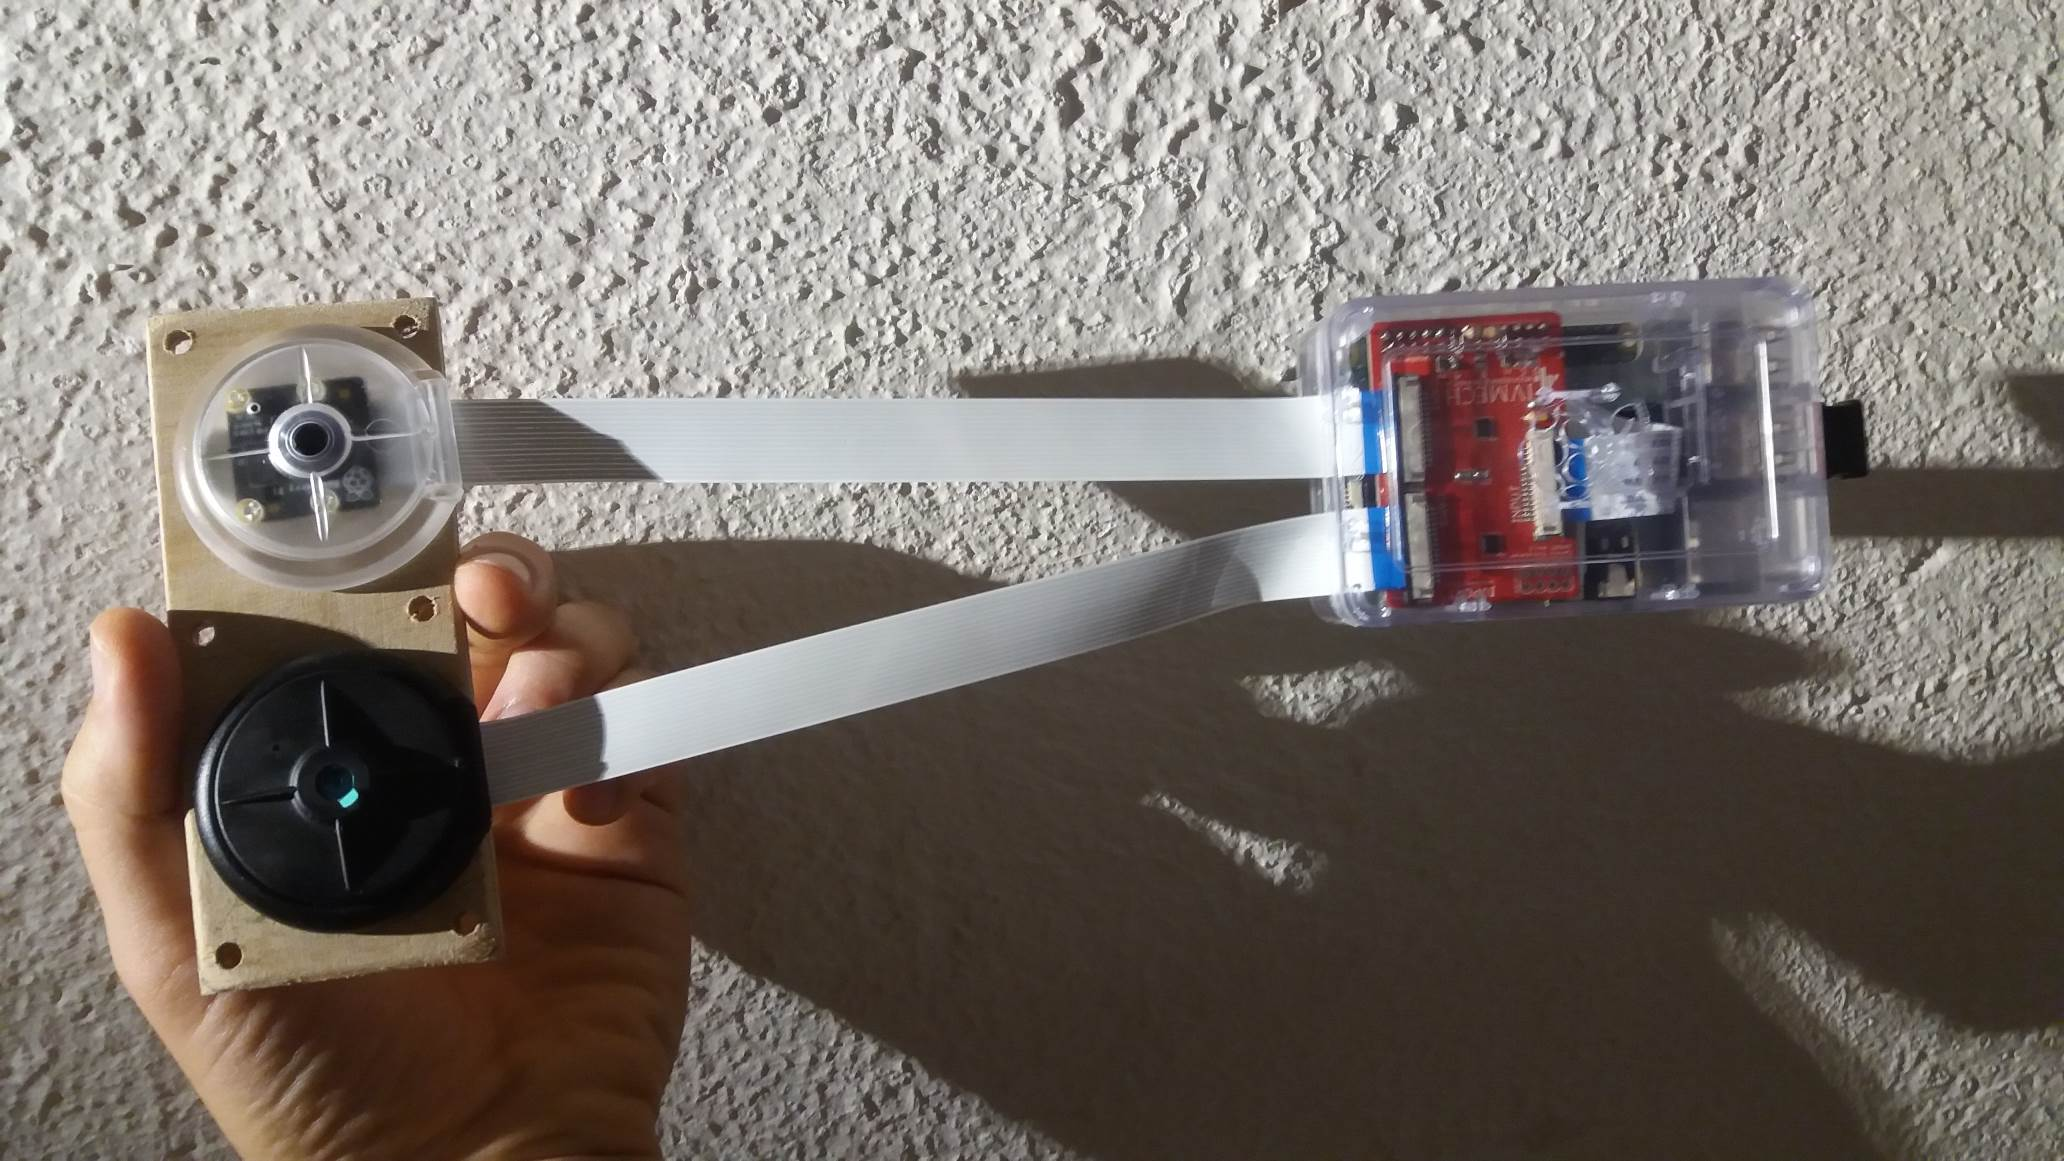
\includegraphics[scale=0.25]{images/ivmech.jpg}
\caption{IVmech camera multiplexer}
\label{fig:ivmech}
\end{figure}

With the dual raspberry pi setup, TCP triggering was used as in code appendix \ref{code:tcp_trigger}, but the overhead and asynchronous nature meant that it was never consistently triggered at the same time. Instead, the clocks are sychronised using NTP, and attempt to trigger every second, on the second. It attempts to, because sometimes the GPU runs garbage collection on its memory to make way for new images. Except for the garbage collection period (which takes a few seconds), the latter solution works quite well, with an occassional few milliseconds difference in stereo captures. This is accounted for in Chapter \ref{sec:image_processing} using feature matching and homography.

\section{The Camera Model}
\label{sec:cam_model}
\subsection{Camera Geometry}
\label{sec:cam_geometry}

It is important to be able to model the cameras in a mathematical form so that unique variances can be accounted for in each camera.\\

The cameras can be approximated as pin-hole camera models with parameters, as in Section \ref{sec:pinhole}. Estimating the parameters is known as 'camera resectioning'. Light enters a camera through its focal point $Fc$, and falls onto the sensor, as depicted in Figure \ref{fig:camera_geometry}. $f$ is the focal length, which is the distance between the image sensor and lens. The symmetry of the model means that $f$ is also the distance between the lens and the image plane, and thus the correct orientation is shown at the image plane.

\begin{figure}[H]
\centering
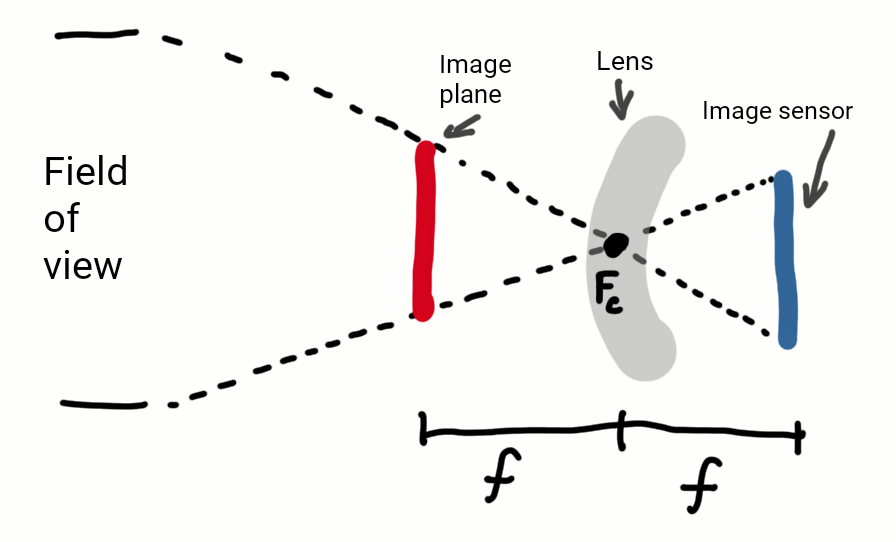
\includegraphics[scale=0.35]{images/camera_geometry.png}
\caption{Geometry of a single camera}
\label{fig:camera_geometry}
\end{figure}

The field of view is restricted by sensor size and focal length, and depends on the distance (or height) of the camera from the subject. Since a stereo setup is used, the field of view overlaps, but not from the same focal point as shown in Figure \ref{fig:stereo_overlap}. The idea would be to superimpose the two image planes one top of each other.

\begin{figure}[H]
\centering
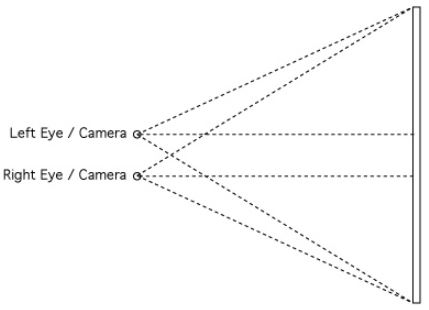
\includegraphics[scale=0.45]{images/stero_overlap.jpg}
\caption{Stereo vision overlap}
\label{fig:stereo_overlap}
\end{figure}

In stereo camears, this is also known as epipolar geometry, where an epipolar plane can be created from the intersection of the two image planes and a 3D point that both cameras are pointing at.

%various coordinate systems?\\
%Cartesian?\\
%right-hand rule?\\
%multiple-cameras used, therefore epiline geometery?\\
%relationship between coordinate systems, camera, image plane, system environment.\\\\
%
%width Xc\\
%height Yc\\
%depth Zc\\
%Focal point Fc set at origin\\
%P exists within R\^3\\\\
%
%image plane provides two coordinate systems, the u-v coordinate system, and the x-y coordinates.\\
%H, W\\
%position of the image plane in conjunction to the cam geometry\\\\
%
%the point at which the principle axis Zc penetrates the image plane is referred to as the principle point and denoted as (Cx, Cy). The principle point is set as the origin of the x-y coordinate system. The point P is bounded within the image plane as so:\\
%Pu, Pv, Px, Py, W, H\\\\
%
%The 3d env defining fields = object space. show origin space relative to other spaces. Focal poitn Fc is aligned\\
%with origin of obj space such that\\
%Zc == Z\\
%obj plane is parallel to the image plane and describes the range of possible X-Y positions of the object at a set distance.\\
%The distance between the focal point and the object plane is workign distance,\\
%denoted as Zd. and can be used to determione the feild of view.\\\\
%
%\subsection{The Camera Model}
%
%camerai is an optical instrument used to capture and store visual info.\\
%the cam model is a mathematical representation of the internal camera geometry\\
%and can be extended to define the position of the camera within the object space.\\
%the camera model is an essential tool used to construct the relation between the camera, image plane and obj space.\\\\
%
%Calibration depends on the info given by the camera model to effectively rectify differences in the stereo setup.\\
%This chapter therefore investigates the construction of the camera model, alogn with the coresponding paramters, to establish how the 3-d object space will be portrayed ion the 2d sapce.\\
%
%The camera model is composed from variuos parameters which are initially unkown The process of identifying or calculating these unkonw params is known as camera calibration.


\subsection{Intrinsic Parameters}
\label{sec:intrinsic}

The internal camera geometry describes the relation between the camera and the image plane. This relation is determined by the focal length, principle point and possible axis misalignment. These defining parameters are referred to as the intrinsic parameters and are measured in pixels.\\

The intrinsic parameters are often represented as a matrix known as the camera matrix. The camera matrix $M_c$ for each camera is defined as:

\begin{equation}\label{eq:cm}
M_c^{(j)}\,=\,\begin{bmatrix}
{f_x^{(j)}} & {s} & {c_x^{(j)}}\\
{0} & {f_y^{(j)}} & {c_y^{(j)}}\\
{0} & {0} & {1}
\end{bmatrix},\quad j = 1,\, 2
\end{equation}

where:\\
$f$ is the focal length\\
$s$ is the skew,\\
and $Cx, Cy$ is the x and y coordinate of the principle point.

\subsection{Extrinsic Parameters}

The extrinsic parameters describe the correspondence between the two camera coordinate systems. The extrinsic parameters include rotation matrix $R$ and translation matrix $T$ to describe how the one coordinate system will map to the other.\\

These intrinsic and extrinsic parameters are used to construct the pin hole camera model.

\subsection{Pinhole Camera model}
\label{sec:pinhole}

The pinhole camera model describes the ideal transformation between a point within the object space and the representation of that point in the image plane. 

%Section 2.3 (cam geometry) provides the description of the pinhole camera concept. 

\begin{figure}[H]
\centering
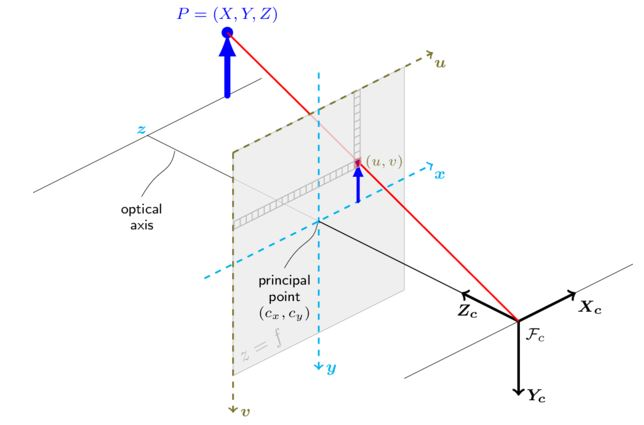
\includegraphics[scale=0.75]{images/pinhole_model.JPG}
\caption{Pinhole camera model \cite{calib3d}}
\label{fig:pinhole_model}	
\end{figure}

The point P is found in figure \ref{fig:pinhole_model} and is defined within the 3d object space as:

\begin{equation}\label{eq:principleP}
P =  \begin{bmatrix}{X}\\{Y}\\{Z}\end{bmatrix}
\end{equation}

The extrinsic parameters are used to describe P in terms of the (x, y, z) coordinate system illustrated in blue in figure.

\begin{equation}\label{eq:principleP_transformation}
\begin{bmatrix}{x}\\{y}\\{z}\end{bmatrix} = R  \begin{bmatrix}{X}\\{Y}\\{Z}\end{bmatrix}\,+\,T\\
\end{equation}

where:\\
$R$ is the rotational matrix\\
$T$ is the translational vector\\

If the extrinsic parameters are known, then:

\begin{align*}
R = I, and\\
T = 0
\end{align*}

and Equation \ref{eq:principleP_transformation} is altered as follows 

\begin{equation}\label{altered}
\begin{bmatrix}{x}\\{y}\\{z}\end{bmatrix} =  \begin{bmatrix}{X}\\{Y}\\{Z}\end{bmatrix}
\end{equation}\\

If the distance $z$ is equal to the focal length $f$, the x-y will represent the 2-D image plane. The representation of P remains unchanged if the the coordinates are multiplied by a common factor. This multiplication conceptually shifts the x-y plane along the principle axis. The representation of point $P$ in equation \ref{altered} is consequently modified as follows:

\begin{equation}x' = x/z,\quad and \end{equation}
\begin{equation}y' = y/z \end{equation}

under the condition that \begin{align*} z \neq 0 \end{align*}

The image plane will therefore represent $P$ in terms of the $u-v$ coordinate system, defined in figure x as 

\begin{equation}\label{eq:uv1}u = f_x*x'' + c_x \\ \end{equation}
\begin{equation}\label{eq:uv2}v = f_y*y'' + c_y \end{equation}

where:\\
$(c_x, c_y)$ is the principle point, and\\
$f$ is the focal length.\\

Equation \ref{eq:uv1} and \ref{eq:uv2} can also be written as:

\begin{equation}
\begin{bmatrix}u\\v\\l\end{bmatrix} =  
\begin{bmatrix}
f & 0 & C_x\\
0 & f & C_y\\
0 & 0 & 1
\end{bmatrix}
\begin{bmatrix}x'\\y'\\1\end{bmatrix}
\end{equation}

The derivation of the camera matrix $M_c$ in equation \ref{eq:cm} is effectively as performed above. The pinhole camera model assumes ideal alignment and therefore no skew is present within the model. This concludes the construction of the camera model.

\section{Camera Stereo-calibration}
\label{sec:cal_technique}

Camera calibration can now be performed to identify the unknown parameters within the camera model.

The calibration technique provided by OpenCV was used to identify the unknown parameters. The tutorial adopts the corner detection calibration method described below.\\

The corner detection calibration method is a common calibration technique due to the simplicity of the calibration process.  A chessboard is used as a reference point for the calibration even if the dimensions are unknown, it can be assume that the squares exist on a 2-D plane in a 3-D space. Multiple images containing various orientations of the chessboard are used to detect the size and orientation of the squares. These measurements are then used to determine the unknown parameters. Figure \ref{fig:rgb_input_chess} and \ref{fig:ir_input_chess} shows how the chessboard is observed by the camera for multiple orientations.\\

Stereo-calibration using 16x16 square chess board images was used as in Appendix \ref{app:chess}.\\

Intrinsic parameters such as the distortion coefficients in Equation \ref{eq:dist}, are known as the radial and tangential coefficients, respectively. They are found from calculating the corresponding corners in the chess image sets.

\begin{equation}\label{eq:dist}
dist\,=\,\begin{bmatrix}
k_1 & k_2 & p_1 & p_2 & k_3
\end{bmatrix}
\end{equation}

Radial distortion can be solved as follows:

\begin{align*}
x_{corrected} = x( 1 + k_1 r^2 + k_2 r^4 + k_3 r^6) \\
y_{corrected} = y( 1 + k_1 r^2 + k_2 r^4 + k_3 r^6)
\end{align*}

Similarly, tangential distortion is solved as below. It occurs because the image taking lens is not aligned perfectly parallel to the imaging plane.

\begin{align*}
x_{corrected} = x + [ 2p_1xy + p_2(r^2+2x^2)] \\
y_{corrected} = y + [ p_1(r^2+ 2y^2)+ 2p_2xy]
\end{align*}

Since the poses of the chess boards relate to the first and second camera, it should be possible to superimpose the images on top of each other if we can find these extrinsic parameters. Given $R_1, T_1$, we only need to know the orientation and position of the second camera relative to the first one. Thus, we compute $R,\ T$ such that:

\begin{align*}R_2=R*R_1\quad\quad T_2=R*T_1 + T \end{align*}

The essential matrix is seen as the precursor to the fundamental matrix, and it can be used to determine both the relative position and orientation between the cameras and the 3D position of corresponding image points if the intrinsic parameters are known:

\begin{align*}
E\,=\,\begin{bmatrix}
{0} & {-T_2} & {T_1}\\
{T_2} & {0} & {-T_0}\\
{-T_1} & {T_0} & {0} 
\end{bmatrix}\,*\,R
\end{align*}

where $T_i$ are the components of the translation vector $T : T=[T_0, T_1, T_2]^T$.\\

The fundamental matrix can be calculated as follows:

\begin{align*}
F = M_{c,2}^{-T}\cdot E\cdot M_{c,1}^{-1} 
\end{align*}

Measured results exist in Appendix \ref{app:stereo_results}.

\section{Stereo-rectification}

Taking the calculations from Section \ref{sec:cal_technique}, we can calculate the projections required to essentially make  both image planes the same.

\begin{align*}
P1 = \begin{bmatrix} f & 0 & cx_1 & 0 \\ 0 & f & cy & 0 \\ 0 & 0 & 1 & 0 \end{bmatrix}
\end{align*}

\begin{align*}
P2 = \begin{bmatrix} f & 0 & cx_2 & T_x*f \\ 0 & f & cy & 0 \\ 0 & 0 & 1 & 0 \end{bmatrix}
\end{align*}

where:\\
$P1$ and $P2$ are the projection matrices,\\
and $T_x$ is a horizontal shift between the two cameras.\\

%%\begin{equation}\label{eq:3}
%\begin{equation}x'' = x'  \frac{1 + k_1 r^2 + k_2 r^4 + k_3 r^6}{1 + k_4 r^2 + k_5 r^4 + k_6 r^6} + 2 p_1 x' y' + p_2(r^2 + 2 x'^2)  \\ \end{equation}
%\begin{equation}y'' = y'  \frac{1 + k_1 r^2 + k_2 r^4 + k_3 r^6}{1 + k_4 r^2 + k_5 r^4 + k_6 r^6} + p_1 (r^2 + 2 y'^2) + 2 p_2 x' y'  \\
%\quad \text{where} \quad r^2 = x'^2 + y'^2  \\ \end{equation}

Measured results exist in Appendix \ref{app:stereo_results}.

\section{Undistortion}
\label{sec:undistortion}

Undistortion of the images is required, as in Figure \ref{fig:distortion_examples}. If the image set is too close to the centre, then an incorrect undistortion occurs as in Figure \ref{fig:incorrectly_undistorted}.

\begin{figure}[H]
\centering
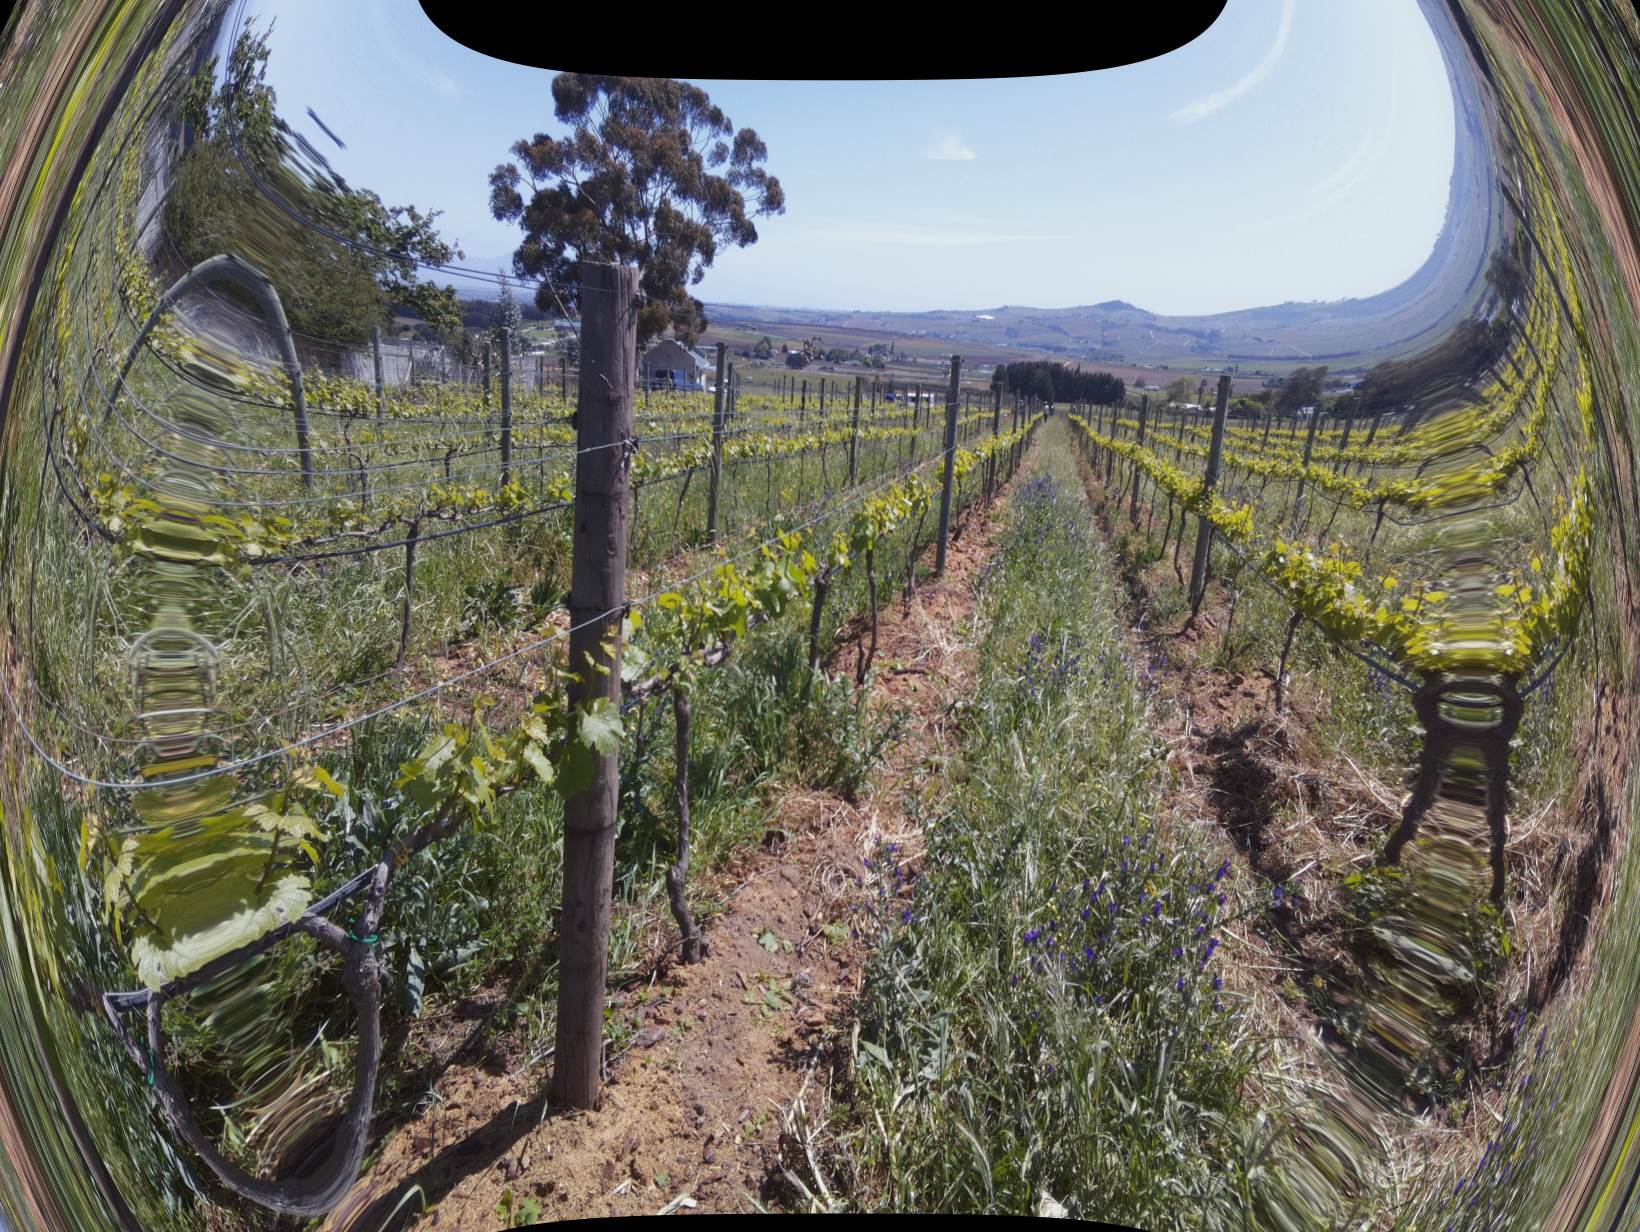
\includegraphics[scale=0.25]{images/incorrectly_undistorted.jpg}
\caption{Undistortion when using 8x8 chessboard image set with images not close enough to the edges}
\label{fig:incorrectly_undistorted}
\end{figure}

In Figure \ref{fig:undistorted_roi}, the 16x16 chess set (Figure \ref{fig:rgb_input_chess} and \ref{fig:ir_input_chess}) was used for stereo-calibration.

\begin{figure}[H]
\begin{subfigure}{0.5\textwidth}
\centering
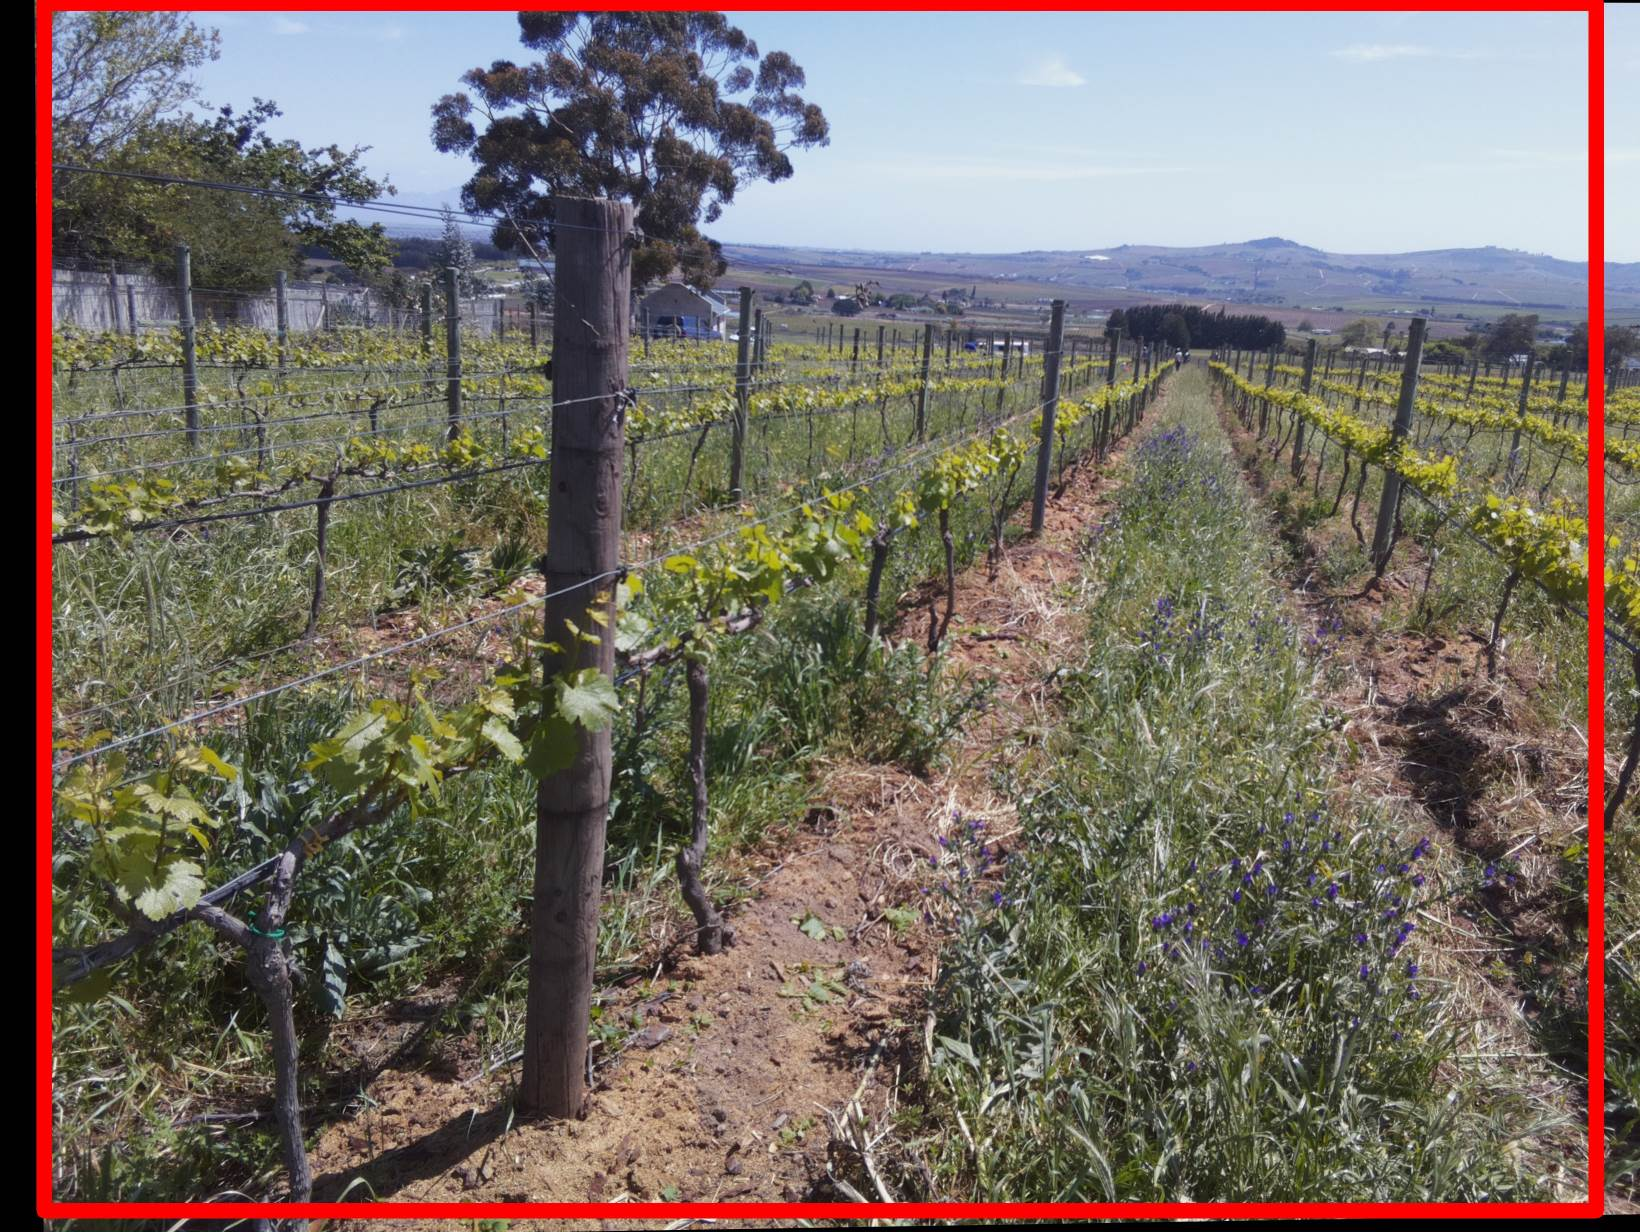
\includegraphics[scale=0.17]{images/rgb_undistorted.jpg}
\caption{RGB image}
\label{fig:rgb_undistorted}
\end{subfigure}
\begin{subfigure}{0.5\textwidth}
\centering
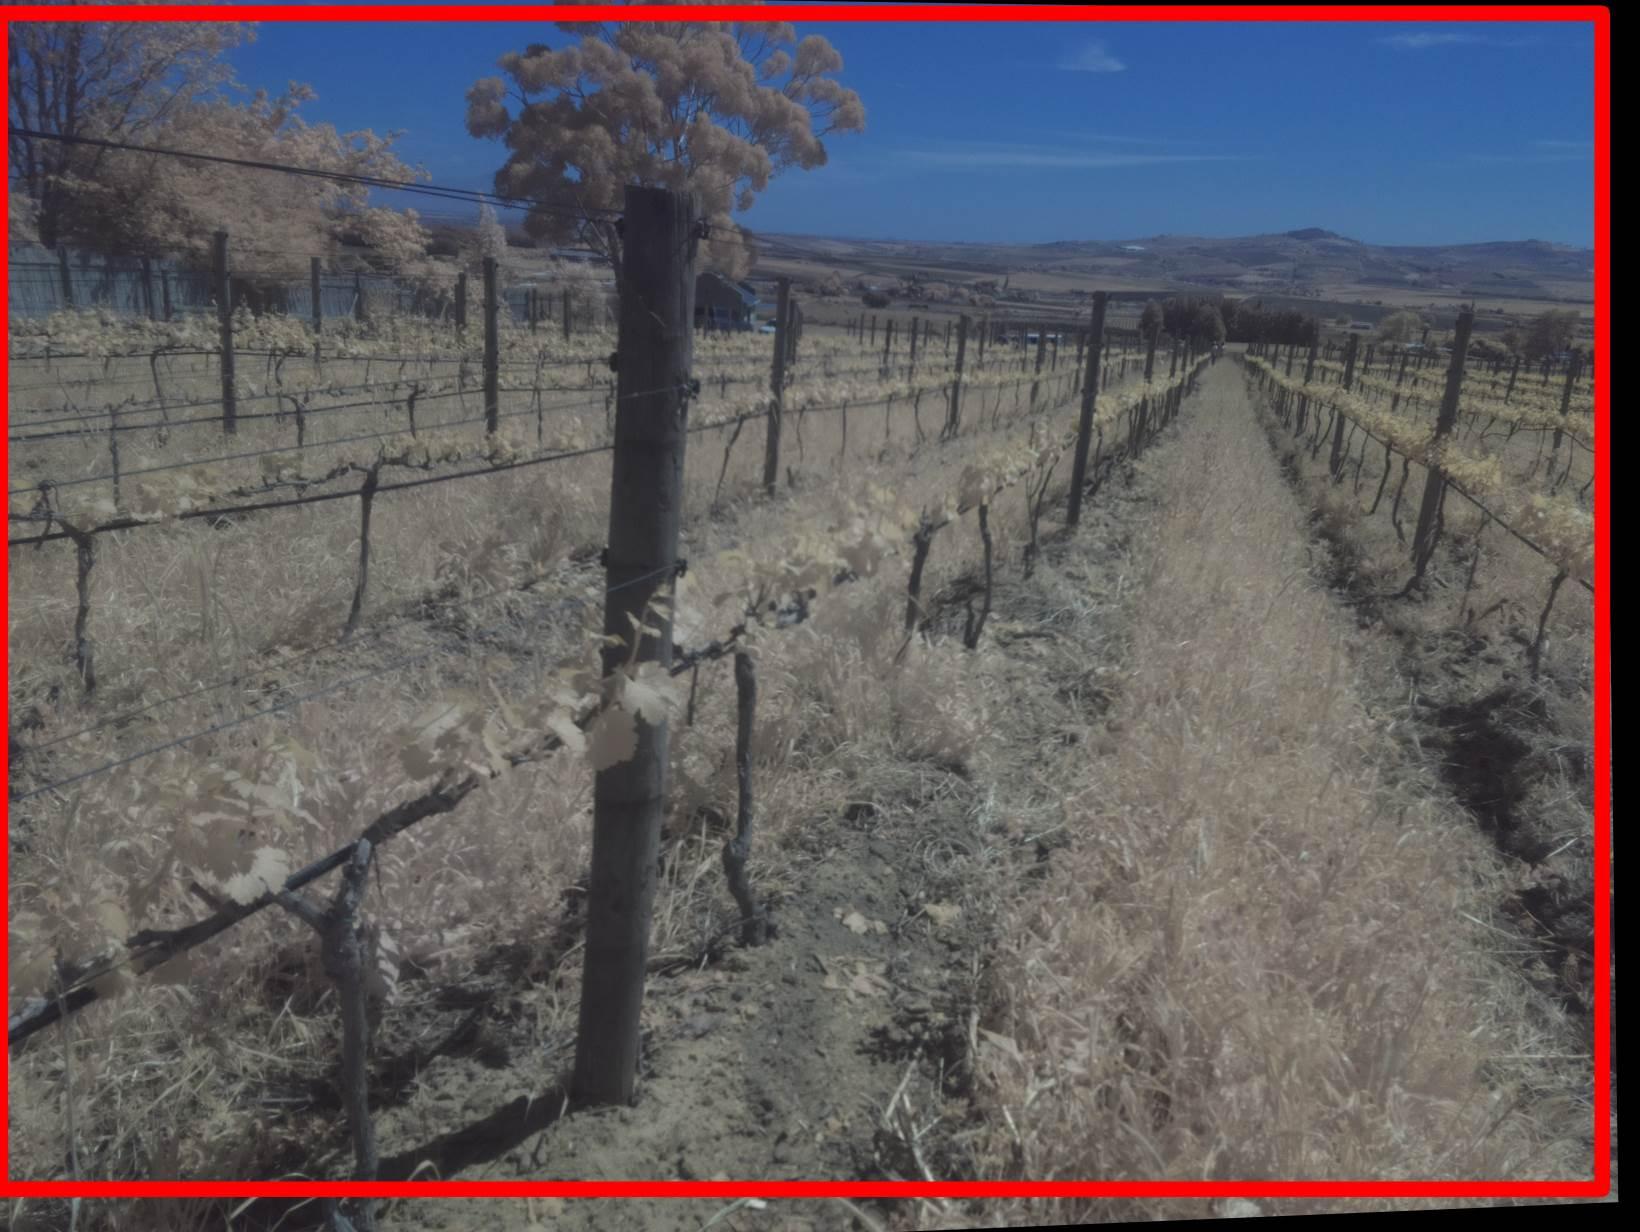
\includegraphics[scale=0.17]{images/ir_undistorted.jpg}
\caption{Corresponding IR image}
\label{fig:ir_undistorted}
\end{subfigure}
\caption{Correctly undistorted images with valid ROI outlined}
\label{fig:undistorted_roi}
\end{figure}